%versi 3 (22-07-2020)
\chapter{Landasan Teori}
\label{chap:teori}

% Reference test
%\cite{mueller:2007:windowscommandline}
%\cite{shottsjr:2019:linuxcommandline}
%\cite{matthew:2007:beginninglinuxprogramming}
%\cite{kerrisk:2010:linuxprogramminginterface}

\section{\textit{Command Line}}
\label{sec:commandline}
\textit{Command line} (atau \cli) dapat diartikan sebagai tampilan antarmuka/\textit{interface} yang memproses perintah dari pengguna dan meneruskannya langsung ke sistem operasi untuk dijalankan.\cite{shottsjr:2019:linuxcommandline} Seluruh sistem operasi komputer yang ada memiliki sebuah \cli dalam bentuk \textit{shell}, yang dapat digunakan oleh penggunanya untuk langsung mengakses fungsi atau servis yang disediakan oleh sistem operasi.\cite{mueller:2007:windowscommandline} 

%Sedangkan, perangkat lunak yang memproses \cli ini disebut sebagai \cl \textit{interpreter}\cite{mueller:2007:windowscommandline} atau \textit{shell}.\cite{shottsjr:2019:linuxcommandline}

\subsection{\textit{Command Line Interface} dan \textit{Graphical User Interface}}
\label{sec:commandline-comparison}

Ada beberapa dari tipe antarmuka yang masih banyak digunakan di zaman sekarang, tetapi dua tipe yang paling banyak muncul adalah \cli dan \gui. Perangkat lunak berbasis \cl sendiri bisa memiliki berbagai macam tampilan, tetapi semuanya selalu mengikuti satu bentuk antarmuka umum. Bentuk yang dimaksud adalah sebuah area/\textit{window} yang memuat teks berupa perintah-perintah dari user untuk dilakukan oleh komputer, beserta keluarannya yang juga berupa teks, seperti dapat dilihat pada gambar \ref{fig:commandline-cli}. Jenis perangkat lunak seperti ini disebut memiliki antarmuka jenis \cli (CLI). Adapun dekorasi visual yang dimiliki oleh jenis tampilan ini hanya berupa warna pada teks-teks yang ada, tanpa tambahan gambar apapun. Jika perangkat lunak tersebut memiliki dekorasi dan/atau tombol interaktif berupa gambar grafis, seperti pada gambar \ref{fig:commandline-gui}, maka perangkat lunak tersebut dikategorikan sebagai perangkat lunak berbasis \gui.

\begin{figure}[ht]
    \begin{subfigure}[b]{0.475\linewidth}
		\centering
		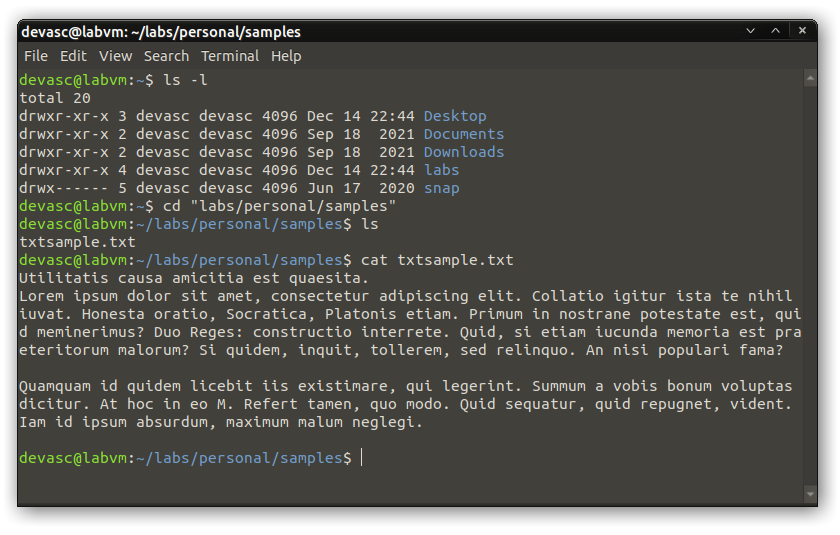
\includegraphics[height=4.7cm]{terminal-linux}
		\caption{Antarmuka perangkat lunak berbasis \cli.}
		\label{fig:commandline-cli}
	\end{subfigure}
	\hfill
    \begin{subfigure}[b]{0.475\linewidth}
		\centering
		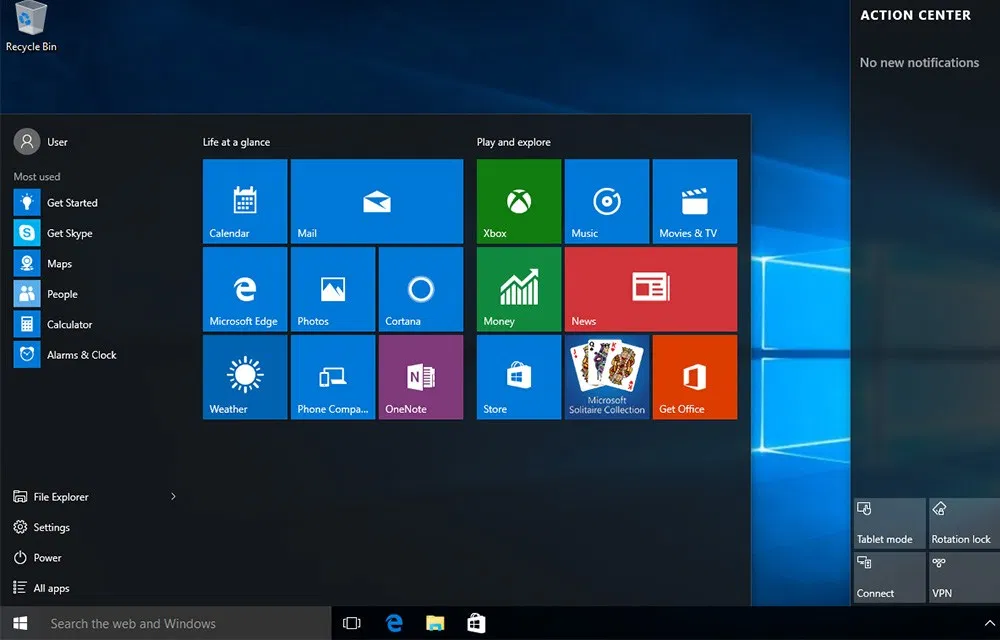
\includegraphics[height=4.5cm]{gui}
		\caption{Antarmuka perangkat lunak berbasis \gui.}
		\label{fig:commandline-gui}
	\end{subfigure}
    \caption[Dua jenis tampilan perangkat lunak]{Contoh dua jenis antarmuka (\textit{interface)} perangkat lunak.}
	\label{fig:commandline-interfacetypes}
\end{figure}

Selain dari tampilannya sendiri, ada beberapa perbedaan utama lain antara perangkat-perangkat lunak berbasis \cli dengan perangkat lunak berbasis \gui. Adapun perbedaan-perbedaan utama dari kedua jenis antarmuka ini adalah sebagai berikut.
\begin{itemize}
	\item Pengunaan sumber daya sistem untuk menjalankan perangkat lunak berbasis \cli lebih rendah dibandingkan dengan perangkat lunak berbasis \gui.
	\item Bagi pengguna pemula (atau pengguna awam pada umumnya), perangkat lunak berbasis \cli akan lebih sulit digunakan karena tidak adanya bantuan apapun dalam bentuk visual, sehingga satu-satunya cara untuk tahu bagaimana cara menggunakan fitur-fiturnya adalah melalui dokumentasi perangkat lunak yang ada. Karena alasan yang sama pula, perangkat lunak berbasis \cli lebih sulit untuk dibiasakan penggunaannya.
	\item Automasi perintah yang bersifat berulan-ulang jauh lebih mudah dilakukan pada perangkat lunak berbasis \cli. Hal ini dikarenakan perangkat lunak berbasis \cli tidak hanya lebih mudah untuk dibuat \textit{script}-nya, tetapi juga lebih efisien untuk digunakan ketika ada banyak sekali perintah yang harus dilakukan pada suatu saat tertentu.\cite{mueller:2007:windowscommandline}
\end{itemize}

\subsection{\textit{Command Line} di Linux}
\label{sec:commandline-linux}

Linux merupakan sebuah sistem operasi yang sangat modular, jadi ada banyak sekali \textit{shell} yang dapat dijalankan dan digunakan di dalamnya. Walaupun begitu, ada satu \textit{shell} yang selalu datang ter-\textit{install} di dalam semua sistem operasi Linux, yaitu \textit{"bash"} (GNU \textit{Bourne Again Shell).}\cite{matthew:2007:beginninglinuxprogramming}

\subsubsection{Tampilan}
\label{sec:commandline-linux-appearance}

Ketika terminal di Linux dijalankan, akan keluar kotak dialog, beserta sebuah baris. Baris ini biasanya berisi sebuah teks dengan format sebagai berikut.

\begin{verbatim}
        <nama pengguna>@<nama perangkat>:<direktori yang sedang diproses>$
\end{verbatim}

Tanda dolar di ujung baris ini menandakan bahwa baris tersebut merupakan baris \textit{shell prompt}, yang merupakan waktu di mana terminal sudah siap menerima masukan dari pengguna untuk diproses. Perlu diingat bahwa di posisi tanda dolar ini, terkadang justru terdapat tanda pagar (\#). Tanda pagar di akhir baris \textit{shell prompt} menandakan bahwa terminal tersebut dijalankan dengan tingkat akses \textit{superuser}, yang berarti bahwa entah pengguna masuk ke sistem sebagai user \textit{root}, atau terminal memiliki izin tingkat \textit{superuser/administrator}.\cite{shottsjr:2019:linuxcommandline}

\begin{figure}[ht]
    \begin{subfigure}[b]{0.475\linewidth}
		\centering
		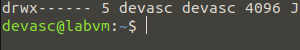
\includegraphics[width=\linewidth]{linux-shellprompt-normal}
		\caption{\textit{Shell prompt} terminal dengan tingkat izin \mbox{normal}.}
		\label{fig:shellprompt-linux-normal}
	\end{subfigure}
	\hfill
    \begin{subfigure}[b]{0.475\linewidth}
		\centering
		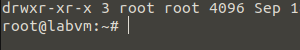
\includegraphics[width=\linewidth]{linux-shellprompt-superuser}
		\caption{\textit{Shell prompt} terminal dengan tingkat izin \textit{\mbox{superuser}}.}
		\label{fig:shellprompt-linux-superuser}
	\end{subfigure}
    \caption{Baris \textit{shell prompt} terminal di sistem operasi Linux.}
	\label{fig:commandline-shellprompt-linux}
\end{figure}

\subsubsection{Navigasi}
\label{sec:commandline-linux-nav}

Sama seperti di Windows, Linux menyimpan file-filenya di sebuah struktur direktori yang bersifat hierarkial. Hal ini berarti bahwa file-file tersebut disimpan dalam direktori-direktori (atau \textit{folder-folder}) yang tersusun seperti sebuah pohon. dalam arti bahwa satu \textit{folder} bisa jadi berada di dalam satu \textit{folder} lain, atau berisi beberapa \textit{folder} lainnya.\cite{shottsjr:2019:linuxcommandline}

Untuk navigasi, terminal Linux memiliki beberapa perintah utama. Adapun perintah-perintah tersebut adalah sebagai berikut.

\begin{itemize}
	\item \verb|pwd| \cite{shottsjr:2019:linuxcommandline}\\
	\verb|pwd| merupakan singkatan dari \textit{print working directory}, yang berarti bahwa perintah ini akan mengeluarkan \textit{working directory}, atau direktori tempat terminal sekarang sedang bekerja/berjalan, sebagai keluaran dari perintah tersebut. Ketika pengguna pertama kali menjalankan terminal, \textit{working directory}-nya selalu merupakan direktori \textit{home} dari perangkat.
	\item \verb|ls| \cite{shottsjr:2019:linuxcommandline}\\
	\verb|ls| digunakan untuk menghasilkan keluaran berupa isi dari folder yang dispesifikasi. Biasanya digunakan ketika pengguna sudah memasuki folder yang diinginkan, walaupun dengan perintah ini, pengguna bisa saja mengintip isi dari folder manapun di direktori manapun, dengan mengikutkan direktori yang diinginkan sebagai parameter dari perintah tersebut. Adapun Isi dari folder yang diikutkan sebagai parameter tidak hanya berupa folder lain, tetapi juga seluruh file-file yang ada, walaupun untuk file-file yang disembunyikan (nama file diawali dengan tanda titik), perlu ditambahkan opsi \verb|-a| agar file-file tersebut muncul pula dalam keluarannya.
	\item \verb|cd| \cite{shottsjr:2019:linuxcommandline}\\
	\verb|cd| adalah perintah yang berfungsi untuk mengganti \textit{working directory} dari terminal. Untuk melakukan hal tersebut, perintah yang perlu dimasukkan adalah sebagai berikut:
	
	\begin{verbatim}
	                     cd <direktori yang diinginkan>
	\end{verbatim}
	
	Direktori yang diinginkan dapat berupa direktori absolut, atau direktori relatif. Perbedaannya adalah direktori absolut selalu dimulai dari folder \textit{root}, mengikuti folder-folder apapun yang ada di antara \textit{root} sampai ke folder yang diinginkan.
	
	Sedangkan, direktori relatif selalu dimulai dari \textit{working directory}. Untuk penggunaan direktori relatif, diperlukan dua buah notasi spesial, yaitu titik (\verb|.|), yang merepresentasikan \textit{working directory} sekarang itu sendiri, dan dua titik (\verb|..|), yang merepresentasikan \textit{parent folder} dari \textit{working directory}.
\end{itemize}

\subsection{\textit{Command Line} di Windows}
\label{sec:commandline-windows}

% Start of block comment (old ver)
\begin{comment}

\subsection{Struktur Perintah \textit{Command Line}}
\label{sec:commandline-commands}

Perangkat lunak \cl memiliki struktur perintah sebagai berikut:\footnote{\href{https://www.gnu.org/savannah-checkouts/gnu/bash/manual/bash.html\#Shell-Commands}{Bash Reference Manual} dan \href{https://docs.microsoft.com/en-us/previous-versions/windows/it-pro/windows-xp/bb490954(v=technet.10)}{Microsoft Docs}}

\begin{quote}
	\centering
	\textit{prompt command parameter1 parameter2 ... parameterN}
\end{quote}

\begin{itemize}
	\item \textit{Prompt} \cite{shottsjr:2019:linuxcommandline} \\
	\textit{Prompt} merupakan keluaran teks dari \cli yang menandakan tempat/waktu di mana \textit{shell} sudah siap untuk menerima input dari pengguna. \textit{Prompt} umumnya berupa karakter tertentu, seperti tanda dolar (\$), tanda pagar (\#), atau tanda kurung sudut kiri (>).\footnote{\href{http://www.cpm.z80.de/manuals/SID86\_User\_Guide.txt}{http://www.cpm.z80.de/manuals/SID86\_User\_Guide.txt}}
	\item \textit{Command} \\
	Merupakan perintah yang diberikan oleh pengguna untuk dijalankan oleh perangkat lunak.
	\item \textit{Parameter} \\
	Parameter yang diberikan oleh pengguna sebagai iringan dari perintah yang diinginkan. Parameter biasanya berupa huruf, kata, atau angka, dan merupakan nilai variabel tambahan yang diperlukan untuk operasi yang akan dilakukan oleh perintah yang dimasukkan sebelumnya. Bersifat opsional, dalam arti bahwa beberapa perintah bisa jadi memerlukan \textit{N}-buah parameter, sedangkan beberapa lainnya tidak perlu parameter apapun.
\end{itemize}

\subsection{Tipe Antarmuka \textit{Command Line}}
\label{sec:commandline-type}

Berdasarkan sumber dari perangkat lunak \cl, antarmuka \cl dibagi menjadi dua, yaitu \cli dari OS dan aplikasi \cli.

\subsubsection{OS (\textit{Built-In})}
\label{sec:commandline-type-os}
Antarmuka \cl tipe ini merupakan antarmuka bawaan, dalam arti bahwa perangkat lunak ini sudah diikutkan dalam instalasi sistem operasi oleh pengguna. Dua contoh dari \cli tipe ini yang paling umum adalah \textit{cmd.exe} dalam sistem operasi Windows dan \textit{bash} dalam sistem operasi Linux.

\subsubsection{Aplikasi}
\label{sec:commandline-type-app}
Antarmuka \cl tipe ini merupakan antarmuka yang datang sebagai fitur dari aplikasi tertentu, baik dari pembuat yang sama dengan sistem operasi yang terdapat di perangkat milik pengguna (tapi bukan bawaan), atau dari pihak ketiga. Tipe ini biasanya banyak ditemukan dalam perangkat lunak zaman dahulu\textemdash spesifiknya, tahun-tahun ketika GUI masih belum merupakan teknologi yang mudah diimplementasikan. Walaupun begitu, pada zaman sekarang pun, masih banyak juga perangkat lunak yang memilih tipe antarmuka CLI dari pada GUI. Salah satu dari contoh aplikasi antarmuka tipe ini adalah Git.
\end{comment}
% End of block comment (old ver)

\section{KIRI}
\label{sec:kiri}

KIRI merupakan sebuah perangkat lunak berbasis web yang berfungsi untuk menyelesaikan (atau setidaknya mengurangi) dampak dari masalah-masalah yang dapat diselesaikan oleh transportasi umum/publik di Indonesia, seperti pemanasan global, kemacetan, atau peningkatan harga bensin. Selain itu, turis mancanegara juga memilih untuk menaiki transportasi umum, karena sarana transportasi tersebut tidak hanya jauh lebih murah, tetapi juga memberikan kesempatan kepada mereka untuk melihat seluk-beluk dari kota-kota yang mereka kunjungi. Walaupun begitu, masih banyak masyarakat lokal sendiri yang segan untuk menaiki transportasi publik, umumnya karena transportasi publik lebih rumit persiapannya dibandingkan dengan transportasi privat, seperti kendaraan pribadi.\footnote{\href{https://projectkiri.github.io/\#about-kiri}{https://projectkiri.github.io/\#about-kiri}}

Di halaman web KIRI, pengguna dapat memasukkan input berupa lokasi awal dan lokasi tujuan dan KIRI akan menghasilkan seluruh langkah yang harus ditempuh oleh pengguna untuk sampai ke lokasi tujuan, dengan menggunakan angkot - termasuk kode angkot mana saja yang harus dinaiki, ataupun seberapa jauh pengguna harus berjalan kaki untuk sampai ke lokasi rute angkot berikutnya.

\subsection{Tampilan}
\label{sec:kiri-appearance}

\subsection{API}
\label{sec:kiri-appearance}


\section{Skripsi}
\label{sec:skripsi} 
 
Rencananya akan diisi dengan penjelasan umum mengenai buku skripsi.

\dtext{11-12} 

\section{\LaTeX}
\label{sec:latex}

Mengapa menggunakan \LaTeX{} untuk buku skripsi dan apa keunggulan/kerugiannya bagi mahasiswa dan pembuat template. 

\dtext{13-14}


\section{Template Skripsi FTIS UNPAR}
\label{sec:template}
 
Akan dipaparkan bagaimana menggunakan template ini, termasuk petunjuk singkat membuat referensi, gambar dan tabel.
Juga hal-hal lain yang belum terpikir sampai saat ini. 
 
\dtext{15-16}

\subsection{Tabel}  
Berikut adalah contoh pembuatan tabel. 
Penempatan tabel dan gambar secara umum diatur secara otomatis oleh \LaTeX{}, perhatikan contoh di file bab2.tex untuk melihat bagaimana cara memaksa tabel ditempatkan sesuai keinginan kita.

Perhatikan bawa berbeda dengan penempatan judul gambar gambar, keterangan tabel harus diletakkan di atas tabel!!
Lihat Tabel~\ref{tab:contoh1} berikut ini:

\begin{table}[H] %atau h saja untuk "kira kira di sini"
	\centering 
	\caption{Tabel contoh}
	\label{tab:contoh1}
	\begin{tabular}{cccc}
		\toprule
		& $v_{start}$ & $\mathcal{S}_{1}$ & $v_{end}$\\

		\midrule
		$\tau_{1}$ & 1 & 12& 20\\
		$\tau_{2}$ & 1 &  & 20\\
		$\tau_{3}$ & 1 & 9 & 20\\
		$\tau_{4}$ & 1 &  & 20\\

		\bottomrule
		
	\end{tabular} 
\end{table}
Tabel~\ref{tab:cthwarna1} dan Tabel~\ref{tab:cthwarna2} berikut ini adalah tabel dengan sel yang berwarna dan ada dua tabel yang bersebelahan. 
\begin{table}[H]
	\begin{minipage}[c]{0.49\linewidth}
		\centering
		\caption{Tabel bewarna(1)}
		\label{tab:cthwarna1}
		\begin{tabular}{ccccc}
			\toprule
			 & $v_{start}$ & $\mathcal{S}_{2}$ & $\mathcal{S}_{1}$ & $v_{end}$\\
			
			\midrule
			$\tau_{1}$ & 1 & 5 \cellcolor{green}& 12& 20\\
			$\tau_{2}$ & 1 & 8 \cellcolor{green}& & 20\\
			$\tau_{3}$ & 1 & 2/8/17 \cellcolor{green}& 9 & 20\\
			$\tau_{4}$ & 1 & \cellcolor{red}& & 20\\
			
			\bottomrule

		\end{tabular}
	\end{minipage}
	\begin{minipage}[c]{0.49\linewidth}
		
		\centering 
		\caption{Tabel bewarna(2)}
		\label{tab:cthwarna2}
		\begin{tabular}{ccccc}
			\toprule
			 & $v_{start}$ & $\mathcal{S}_{1}$ & $\mathcal{S}_{2}$ & $v_{end}$\\
			
			\midrule
			$\tau_{1}$ & 1 & 12& 5 \cellcolor{red} &20\\
			$\tau_{2}$ & 1 &  &  8 \cellcolor{green} &20\\
			$\tau_{3}$ & 1 & 9 & 2/8/17 \cellcolor{green} &20\\
			$\tau_{4}$ & 1 &   & \cellcolor{red} &20\\
			
			\bottomrule
		
		\end{tabular}
	\end{minipage}
\end{table}

 
\subsection{Kutipan}
\label{subs:kutipan} 
Berikut contoh kutipan dari berbagai sumber, untuk keterangan lebih lengkap, silahkan membaca file referensi.bib yang disediakan juga di template ini.
Contoh kutipan:
\begin{itemize}
	\item Buku:~\cite{berg:08:compgeom} 
	\item Bab dalam buku:~\cite{kreveld:04:GIS}
	\item Artikel dari Jurnal:~\cite{buchin:13:median}
	\item Artikel dari prosiding seminar/konferensi:~\cite{kreveld:11:median}
	\item Skripsi/Thesis/Disertasi:~\cite{lionov:02:animasi}~\cite{wiratma:10:following}~\cite{wiratma:22:later}
	\item Technical/Scientific Report:~\cite{kreveld:07:watertight}
	\item RFC (Request For Comments):~\cite{RFC1654}
	\item Technical Documentation/Technical Manual:~\cite{Z.500}~\cite{unicode:16:stdv9}~\cite{google:16:and7}
	\item Paten:~\cite{webb:12:comm}
	\item Tidak dipublikasikan:~\cite{wiratma:09:median}~\cite{lionov:11:cpoly}
	\item Laman web:~\cite{erickson:03:cgmodel}  
	\item Lain-lain:~\cite{agung:12:tango}
\end{itemize}    
  
\subsection{Gambar}

Pada hampir semua editor, penempatan gambar di dalam dokumen \LaTeX{} tidak dapat dilakukan melalui proses {\it drag and drop}.
Perhatikan contoh pada file bab2.tex untuk melihat bagaimana cara menempatkan gambar.
Beberapa hal yang harus diperhatikan pada saat menempatkan gambar:
\begin{itemize}
	\item Setiap gambar {\bf harus} diacu di dalam teks (gunakan {\it field} {\sc label})
	\item {\it Field} {\sc caption} digunakan untuk teks pengantar pada gambar. Terdapat dua bagian yaitu yang ada di antara tanda $[$ dan $]$ dan yang ada di antara tanda $\{$ dan $\}$. Yang pertama akan muncul di Daftar Gambar, sedangkan yang kedua akan muncul di teks pengantar gambar. Untuk skripsi ini, samakan isi keduanya.
	\item Jenis file yang dapat digunakan sebagai gambar cukup banyak, tetapi yang paling populer adalah tipe {\sc png} (lihat Gambar~\ref{fig:ularpng}), tipe {\sc jpg} (Gambar~\ref{fig:ularjpg}) dan tipe {\sc pdf} (Gambar~\ref{fig:ularpdf})
	\item Besarnya gambar dapat diatur dengan {\it field} {\sc scale}.
	\item Penempatan gambar diatur menggunakan {\it placement specifier} (di antara tanda  $[$ dan $]$ setelah deklarasi gambar.
	Yang umum digunakan adalah {\bf H} untuk menempatkan gambar {\bf sesuai} penempatannya di file .tex atau  {\bf h} yang berarti "kira-kira" di sini. \\
	Jika tidak menggunakan {\it placement specifier}, \LaTeX{} akan menempatkan gambar secara otomatis untuk menghindari bagian kosong pada dokumen anda.
	Walaupun cara ini sangat mudah, hindarkan terjadinya penempatan dua gambar secara berurutan. 	
	\begin{itemize}
		\item Gambar~\ref{fig:ularpng} ditempatkan di bagian atas halaman, walaupun penempatannya dilakukan setelah penulisan 3 paragraf setelah penjelasan ini.
		\item Gambar~\ref{fig:ularjpg} dengan skala 0.5 ditempatkan di antara dua buah paragraf. Perhatikan penulisannya di dalam file bab2.tex!
		\item Gambar~\ref{fig:ularpdf} ditempatkan menggunakan {\it specifier} {\bf h}.
	\end{itemize}
\end{itemize}
 
\dtext{17-18}
\begin{figure} 
	\centering  
	\includegraphics[scale=1]{ular-png}  
	\caption[Gambar {\it Serpentes} dalam format png]{Gambar {\it Serpentes} dalam format png} 
	\label{fig:ularpng} 
\end{figure} 

\dtext{19-20}
\begin{figure}[H]
	\centering  
	\includegraphics[scale=0.5]{ular-jpg}  
	\caption[Ular kecil]{Ular kecil} 
	\label{fig:ularjpg} 
\end{figure} 
\dtext{21-22}

\begin{figure}[ht] 
	\centering  
	\includegraphics[scale=1]{ular-pdf}  
	\caption[ {\it Serpentes} betina]{ {\it Serpentes} jantan} 
	\label{fig:ularpdf} 
\end{figure} 
 
\subsection{Kode Program}

Kode program dalam bahasa tertentu seringkali harus ditulis di dalam bab, bukan hanya dilampirkan di bagian Lampiran. 
Kode~\ref{kode:aneh} menampilkan penggunaan karakter-karakter yang umum digunakan dalam sebuah program yang ditulis dengan bahasa C.


\begin{lstlisting}[language=Java, caption=Kode untuk menampilkan karakter-karakter aneh, label=kode:aneh]
// This does not make algorithmic sense, 
// but it shows off significant programming characters.

#include<stdio.h>

void myFunction( int input, float* output ) {
	switch ( array[i] ) {
		case 1: // This is silly code
			if ( a >= 0 || b <= 3 && c != x )
				*output += 0.005 + 20050;
			char = 'g';
			b = 2^n + ~right_size - leftSize * MAX_SIZE;
			c = (--aaa + &daa) / (bbb++ - ccc % 2 );
			strcpy(a,"hello $@?"); 
	}
	count = ~mask | 0x00FF00AA;
}

// Fonts for Displaying Program Code in LATEX
// Adrian P. Robson, nepsweb.co.uk
// 8 October 2012
// http://nepsweb.co.uk/docs/progfonts.pdf

\end{lstlisting}

\subsection{Notasi}

Simbol-simbol (matematika) yang sering digunakan sepanjang penulisan skripsi, dapat dimasukkan ke dalam ``Daftar Notasi''. Daftar ini ada di halaman depan sebelum Bab~\ref{chap:intro}.
Cara memasukkan sebuah simbol ke dalam Daftar Notasi adalah menggunakan perintah \verb|\nomenclature|. Contoh:
\begin{center}
    \verb|\nomenclature[]{$A$}{luas kandang ular}|    
\end{center}
\nomenclature[]{$A$}{luas kandang ular}
\nomenclature[]{$n$}{banyaknya ular}
\nomenclature[]{$k$}{jumlah kepala per seekor ular\nomrefpage}
Argumen opsional digunakan untuk mengurutkan notasi. Silahkan lihat sendiri dokumentasi package \verb|nomencl|

